\section{Silicon-tungsten SiD ECal}
\label{sec:Calorimeter:SiliconTungstenSiD}
Most recent update: 2020-05-14 \\
Contacts: Marty Breidenbach, Jim Brau\\ (email: mib@slac.stanford.edu, jimbrau@uoregon.edu)

\subsection{Introduction}
The Silicon Detector (SiD) is a general purpose detector\cite{Behnke:2013lya} designed to conduct precision physics measurements of high energy $e^+e^-$ collisions at the International Linear Collider (ILC). The baseline design uses a Particle Flow Algorithm-based (PFA) approach to reach the jet energy measurement resolution goal of 3\% or better. The major calorimetry challenge imposed by the PFA approach is not the intrinsic calorimetric energy measurement of either the electromagnetic calorimeter (ECal) or the hadronic calorimeter (HCal), but the association of energy deposits with either charged or neutral particles entering the calorimeter (see Figure~\ref{fig:Calorimeter:SiDECAL:showers}). This results in several requirements on the calorimeter design:
\begin{enumerate}[label=\alph*)]
\item To minimize the lateral size of electromagnetic showers, the  Moli\`{e}re  radius  of  the  ECal must be minimized. This enables efficient separation between photons and electrons and charged hadron tracks.
\item Both ECal and HCal must have imaging capabilities which allow assignment of energy cluster deposits to charged or neutral particles. This implies that the readout of both calorimeters needs to be finely segmented transversely and longitudinally.
\item The calorimeter needs to be extendable to small forward angles to ensure hermeticity.
\end{enumerate}

The solution to these requirements is a silicon-tungsten ECal under development. It has a
longitudinal structure of thirty layers - first twenty with a \SI{2.50}{mm} tungsten alloy thickness and \SI{1.25}{mm} readout gap, followed by ten with \SI{5.00}{mm} tungsten alloy plus the same \SI{1.25}{mm} readout gap. The total depth is 26 X$_0$, providing good containment for high energy electromagnetic showers. Simulations have shown the energy resolution for electrons or photons to be well described by 0.17 / $\sqrt{E}$~ $\oplus$ 0.009, degrading some at higher energies
and angles due to changes in sampling
fraction and a small leakage.

\begin{figure}
	\centering
	\begin{minipage}[b]{.24\textwidth}
		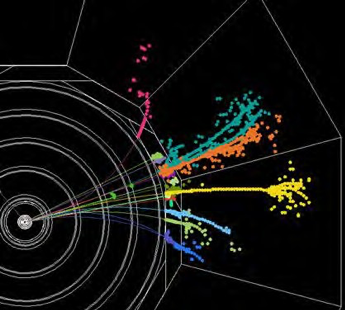
\includegraphics[width=\linewidth,valign=t]{Calorimeter/SiliconTungstenSiD/showers.png}
		\caption{SiD simulation showing tracks and calorimeter activity associated by the PFA algorithm.}
		\label{fig:Calorimeter:SiDECAL:showers}
	\end{minipage}\hfill
	\begin{minipage}[b]{.34\textwidth}
		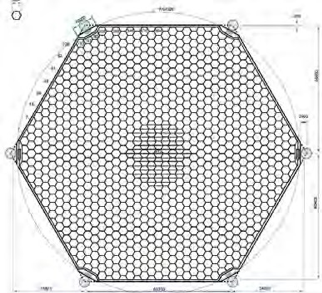
\includegraphics[width=\linewidth,valign=t]{Calorimeter/SiliconTungstenSiD/sensor-drawing.png}
		\caption{Drawing of an individual silicon sensor, segmented into 1024 pixels of \SI{13}{\milli\meter\squared} each}
		\label{fig:Calorimeter:SiDECAL:sensor-drawing}
	\end{minipage}\hfill
	\begin{minipage}[b]{.39\textwidth}
		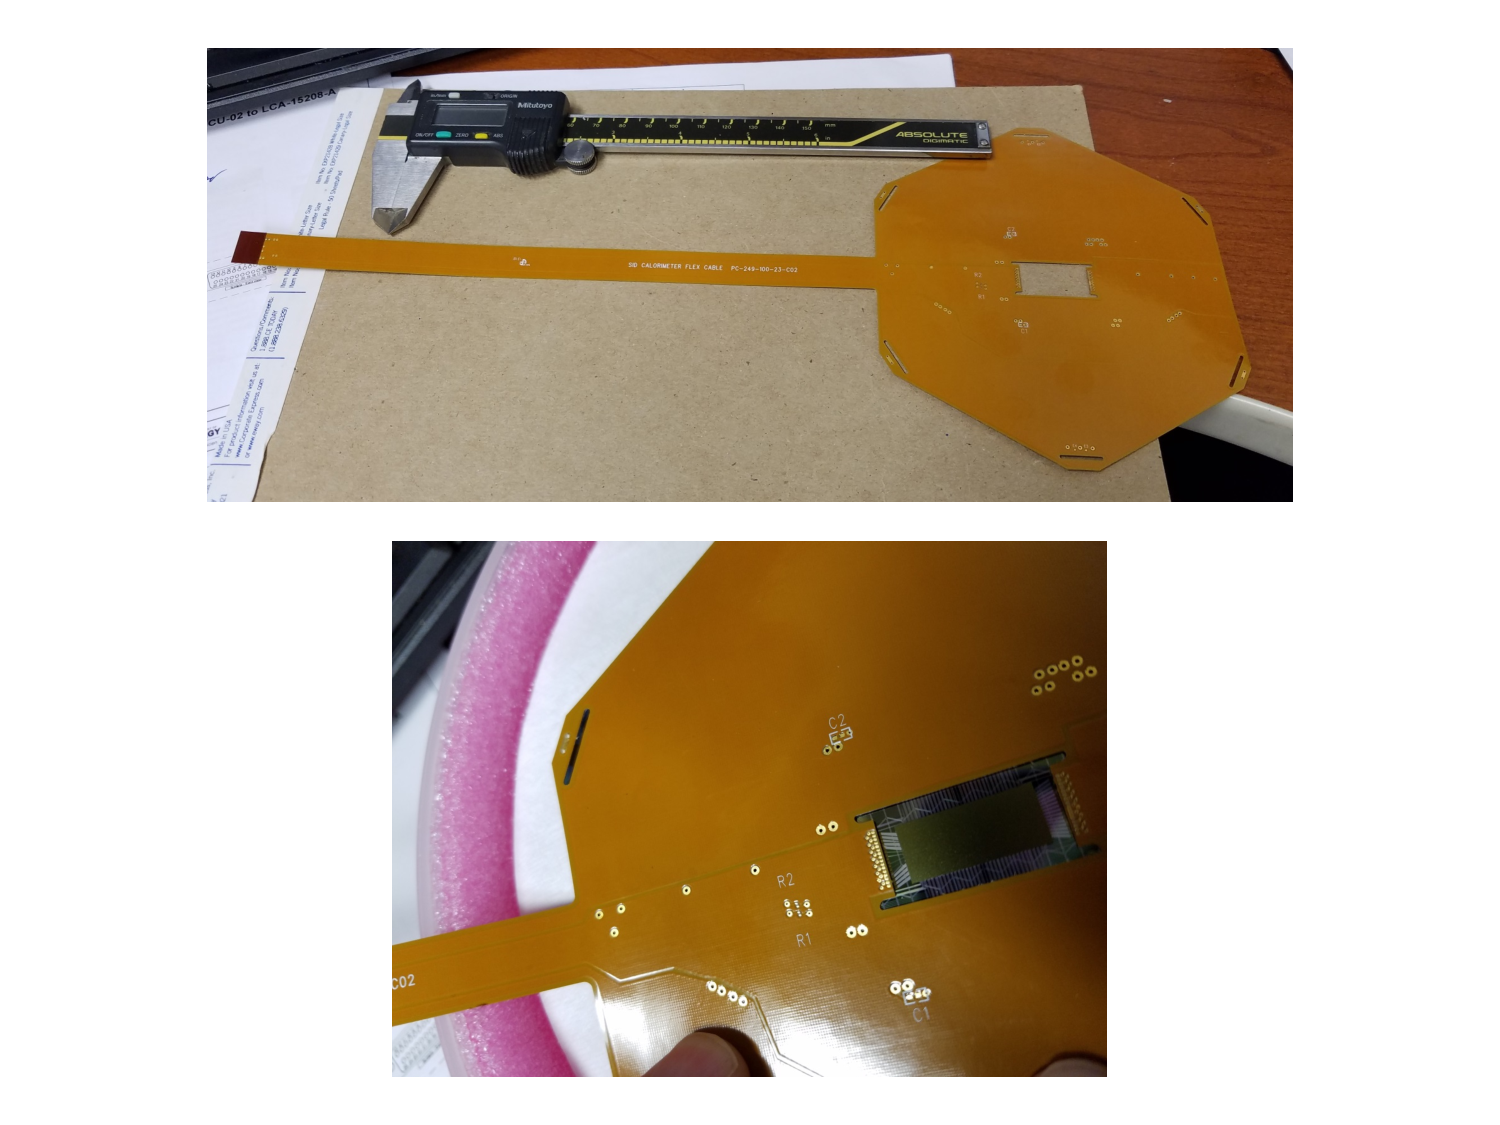
\includegraphics[width=\linewidth,valign=t]{Calorimeter/SiliconTungstenSiD/flex.pdf}
		%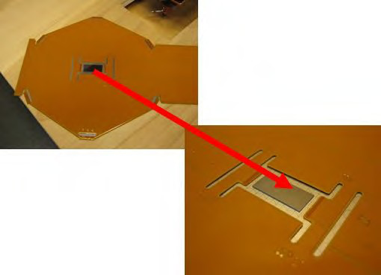
\includegraphics[width=\linewidth,valign=t]{Calorimeter/SiliconTungstenSiD/bonded-sensor.png}
		\caption{Photograph of a fully bonded sensor. The KPiX chip is bump-bonded to the sensor. Power, control and readout signals are provided
via the kapton cable.}
		\label{fig:Calorimeter:SiDECAL:bonded-sensor}
	\end{minipage}
\end{figure}    
               
\subsection{Recent Milestones}
\subsubsection{Sensor and Readout Technology}
In the baseline design, the ECal readout layers are tiled by large, commercially produced silicon sensors (currently assuming 15 cm wafers). The sensors are segmented into pixels which are individually read out over the full range of charge depositions. The complete electronics for the pixels is contained in a single chip, the KPiX ASIC\cite{Brau:2013yb}, which is bump bonded to the wafer. The low beam-crossing duty cycle (10$^{-3}$) of the ILC enables reduction of the heat load using power pulsing, allowing passive thermal management within the ECal modules. Figure~\ref{fig:Calorimeter:SiDECAL:sensor-drawing} shows a sensor with 1024 pixels. 
The pixels are DC-coupled to the KPiX, requiring only two metallization layers for the sensors.
Signal traces are not shown in the figure, but are part of the second layer metallization of the sensors, which connect the pixels to a bump-bonding pad at the center of the sensor for input to the KPiX readout chip.  The pixels near the bump-bonding array at the center are split to reduce capacitance from the large number of signal traces near the sensor center. Electronic noise due to the resistance and capacitance of the traces has been minimized within the allowed trace parameters. Cutouts at the sensor corners accommodate mechanical stand-offs to support gaps between the tungsten layers.


\subsubsection{Bonded Sensor Results}
Bench tests of the KPiX bonded sensor of Figure~\ref{fig:Calorimeter:SiDECAL:bonded-sensor} with a cosmic ray telescope trigger yielded the distribution of maximum charge pixels of Figure~\ref{fig:Calorimeter:SiDECAL:cosmic}. Red and blue distributions show the response of sensor inside
and outside the telescope acceptance.
A Landau distribution (black) is fit to the red signal. The peak of the signal at about \SI{4}{fC} is consistent expectation for minimum-ionizing particles (MIP) passing through the fully-depleted \SI{320}{\micro\meter} thick sensors.
Crosstalk between channels is a potential of the highly integrated design.
Figure~\ref{fig:Calorimeter:SiDECAL:cross-talk} indicates no evidence for crosstalk in any other channel when a large \SI{500}{fC} signal is injected. The noise distribution is nicely fit by a gaussian with RMS \SI{0.2}{fC}. This is to be compared with the \SI{4}{fC} MIP signal. This noise level exceeds the ECal requirements.

\begin{figure}
	\centering
	\hspace*{\fill}
	\begin{minipage}[b]{.45\textwidth}
		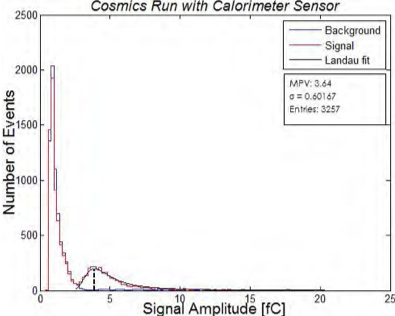
\includegraphics[width=\linewidth,valign=t]{Calorimeter/SiliconTungstenSiD/cosmic.png}
		\caption{Distribution of charge depositions in a bonded sensor for cosmic ray triggered events. The MIP signal is clearly visible above the noise.}
		\label{fig:Calorimeter:SiDECAL:cosmic}
	\end{minipage}\hfill
	\begin{minipage}[b]{.36\textwidth}
		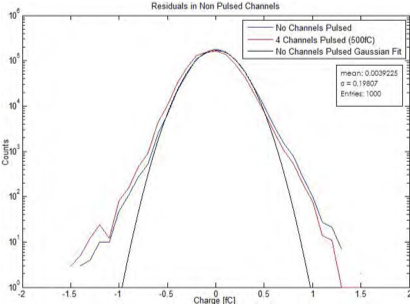
\includegraphics[width=\linewidth,valign=t]{Calorimeter/SiliconTungstenSiD/cross-talk.png}
		\caption{Crosstalk test of a bonded sensor. Charge distributions for all non-pulsed
	pixels compared for a large pulse injection
(red) and no pulse injection (blue).
Also shown gaussian fit with RMS \SI{0.2}{fC}.}
		\label{fig:Calorimeter:SiDECAL:cross-talk}
	\end{minipage}
	\hspace*{\fill}
\end{figure}

\subsubsection{Overall Mechanical Design}
Figure~\ref{fig:Calorimeter:SiDECAL:ECalBarrel} displays the overall mechanical structure of the ECal barrel, showing the overlapping stave geometry designed to minimize uninstrumented regions, especially projective gaps. Figure~\ref{fig:Calorimeter:SiDECAL:wedge} depicts a cross-sectional view of the readout gap in the vicinity of the center of a wedge module. The Kapton flex cables connect near the center of the sensors, bringing power and control signals into the KPiX chip and returning the single 1024 channel digital output line. The signals are multiplexed at the ends of the modules. Cables are being redesigned to service only one sensor at a time, simplifying mechanical assembly but requiring about ten variants of the basic cable design.

 Thermal management is crucial. The KPiX chip has an average power less than \SI{20}{mW}, resulting in a total heat load per wedge module of \SI{115}{W}. A cold plate with water pipes routed laterally at the outside of the wedge (Figure~\ref{fig:Calorimeter:SiDECAL:ECalWedge}) yields a maximum temperature differential of \SI{1.35}{\celsius}.

\begin{figure}
	\centering
	\hspace*{\fill}
	\begin{minipage}[b]{.35\textwidth}
		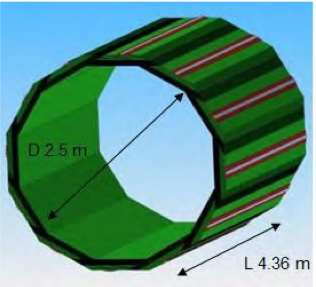
\includegraphics[width=\linewidth,valign=t]{Calorimeter/SiliconTungstenSiD/ECalBarrel.png}
		\caption{ECal Barrel}
		\label{fig:Calorimeter:SiDECAL:ECalBarrel}
	\end{minipage}\hfill
	\begin{minipage}[b]{.43\textwidth}
		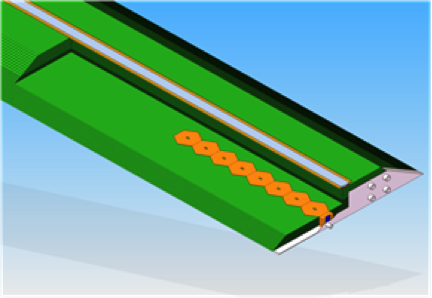
\includegraphics[width=\linewidth,valign=t]{Calorimeter/SiliconTungstenSiD/wedge.png}
		\caption{Cutaway of the SiD ECAL Barrel wedge,
showing the Si sensor and readout cable layout.}
		\label{fig:Calorimeter:SiDECAL:wedge}
	\end{minipage}
	\hspace*{\fill}
\end{figure}


The ECal is built on the first layer of the HCal, which serves as a support and
stiffener, shown in purple
in Figure~\ref{fig:Calorimeter:SiDECAL:ECalWedge}. The active area of the modules have only small gaps for assembly and tolerances; all services are at the
module ends. The HCal plates are tied together by interlaced grooved straps as shown in Figure~\ref{fig:Calorimeter:SiDECAL:HCal-ECal}. The lower HCal plate ``belongs'' to the ECal module. The ECal tungsten plates are tied together with screws and spacers that align with open areas of the sensors.

\begin{figure}
	\centering
	\begin{minipage}[b]{.75\textwidth}
		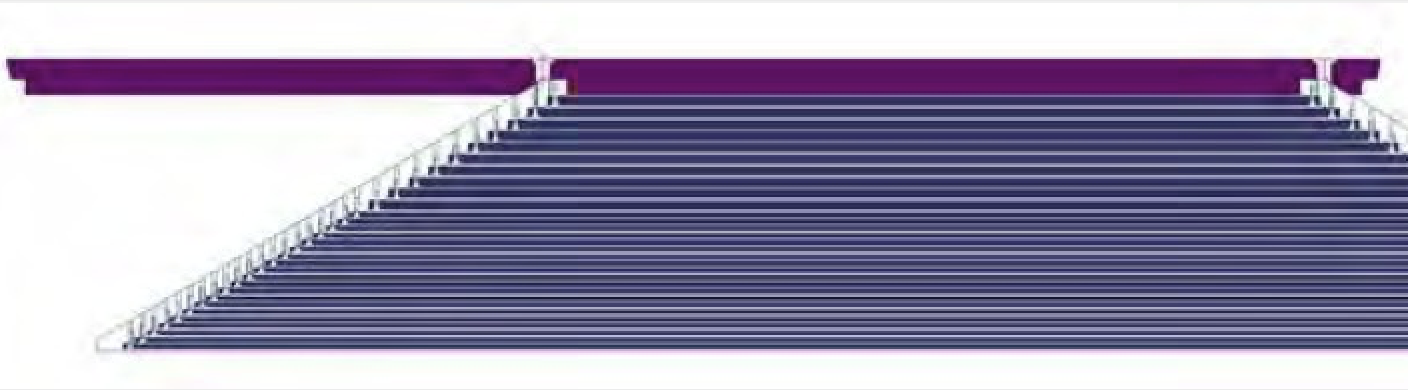
\includegraphics[width=\linewidth,valign=t]{Calorimeter/SiliconTungstenSiD/ECalWedge.png}
		\caption{SiD ECal Barrel wedge, showing the cooling elements (in white) located at the outer radius of the barrel. More details are shown in Figure~\ref{fig:Calorimeter:SiDECAL:HCal-ECal}.}
		\label{fig:Calorimeter:SiDECAL:ECalWedge}
	\end{minipage}\hfill
	\begin{minipage}[b]{.23\textwidth}
		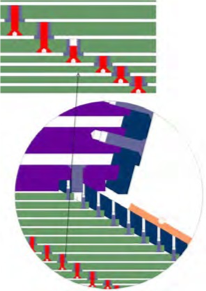
\includegraphics[width=\linewidth,valign=t]{Calorimeter/SiliconTungstenSiD/HCal-ECal.png}
		\caption{Bottom of HCal module with screws and spacers
for ECal tungsten plates. Cooling plate shown in orange at lower right.}
		\label{fig:Calorimeter:SiDECAL:HCal-ECal}
	\end{minipage}
\end{figure}

\subsubsection{Prototype Module and Test Beam}
Based on the positive initial results of the first bonded sensors, and to demonstrate the feasibility of assembling a highly compact electromagnetic calorimeter without printed circuit boards and direct bonding of chips to wafers, a first prototype stack for an SiD ECal has been constructed. This aggressive design has an active gap between  absorber  plates of \SI{1.25}{mm} (Figure~\ref{fig:Calorimeter:SiDECAL:gap}), a cell size of \SI{13}{\milli\meter\squared}, an effective Moliere radius of \SI{14}{mm}, and a width of one sensor. A section of this SiD ECal with KPiX readout was exposed to a \SI{12.1}{GeV} electron  beam  at the SLAC End Station (A) Test Beam Facility. A photo of the test setup is shown in Figure~\ref{fig:Calorimeter:SiDECAL:setup}.

\begin{figure}
	\centering
	\begin{minipage}[b]{.44\textwidth}
		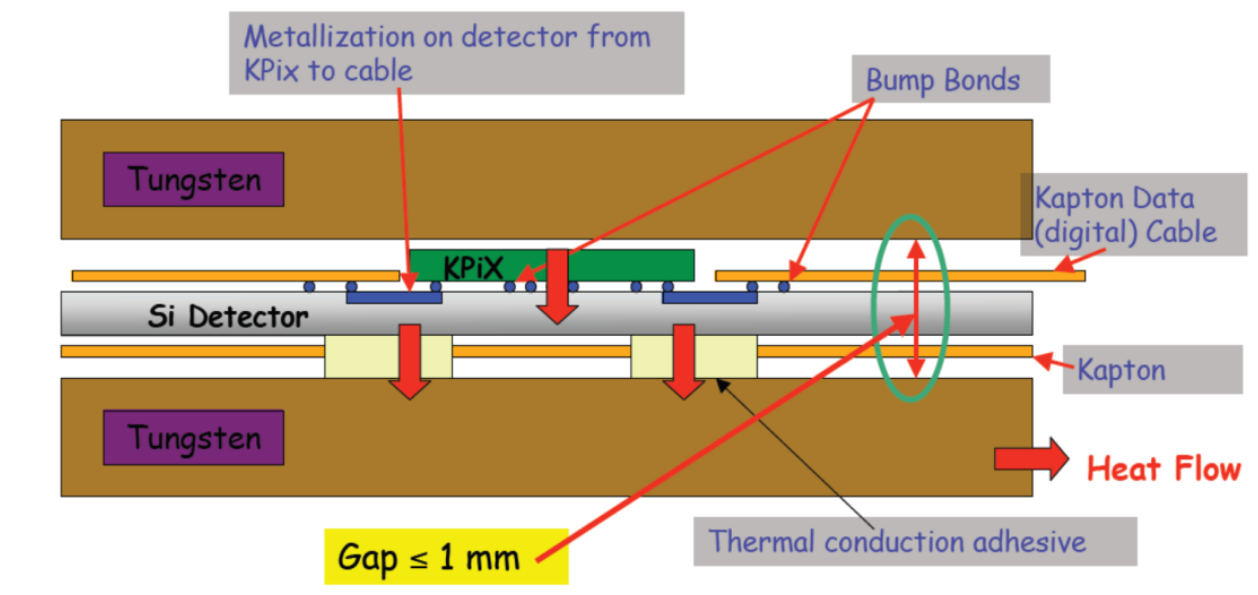
\includegraphics[width=\linewidth,valign=t]{Calorimeter/SiliconTungstenSiD/gap.png}
		\caption{The 1.25 mm gap between tungsten absorber layers includes a 0.3 mm silicon sensor layer bump-bonded to the KPiX readout chip.}
		\label{fig:Calorimeter:SiDECAL:gap}
	\end{minipage}\hfill
	\begin{minipage}[b]{.44\textwidth}
		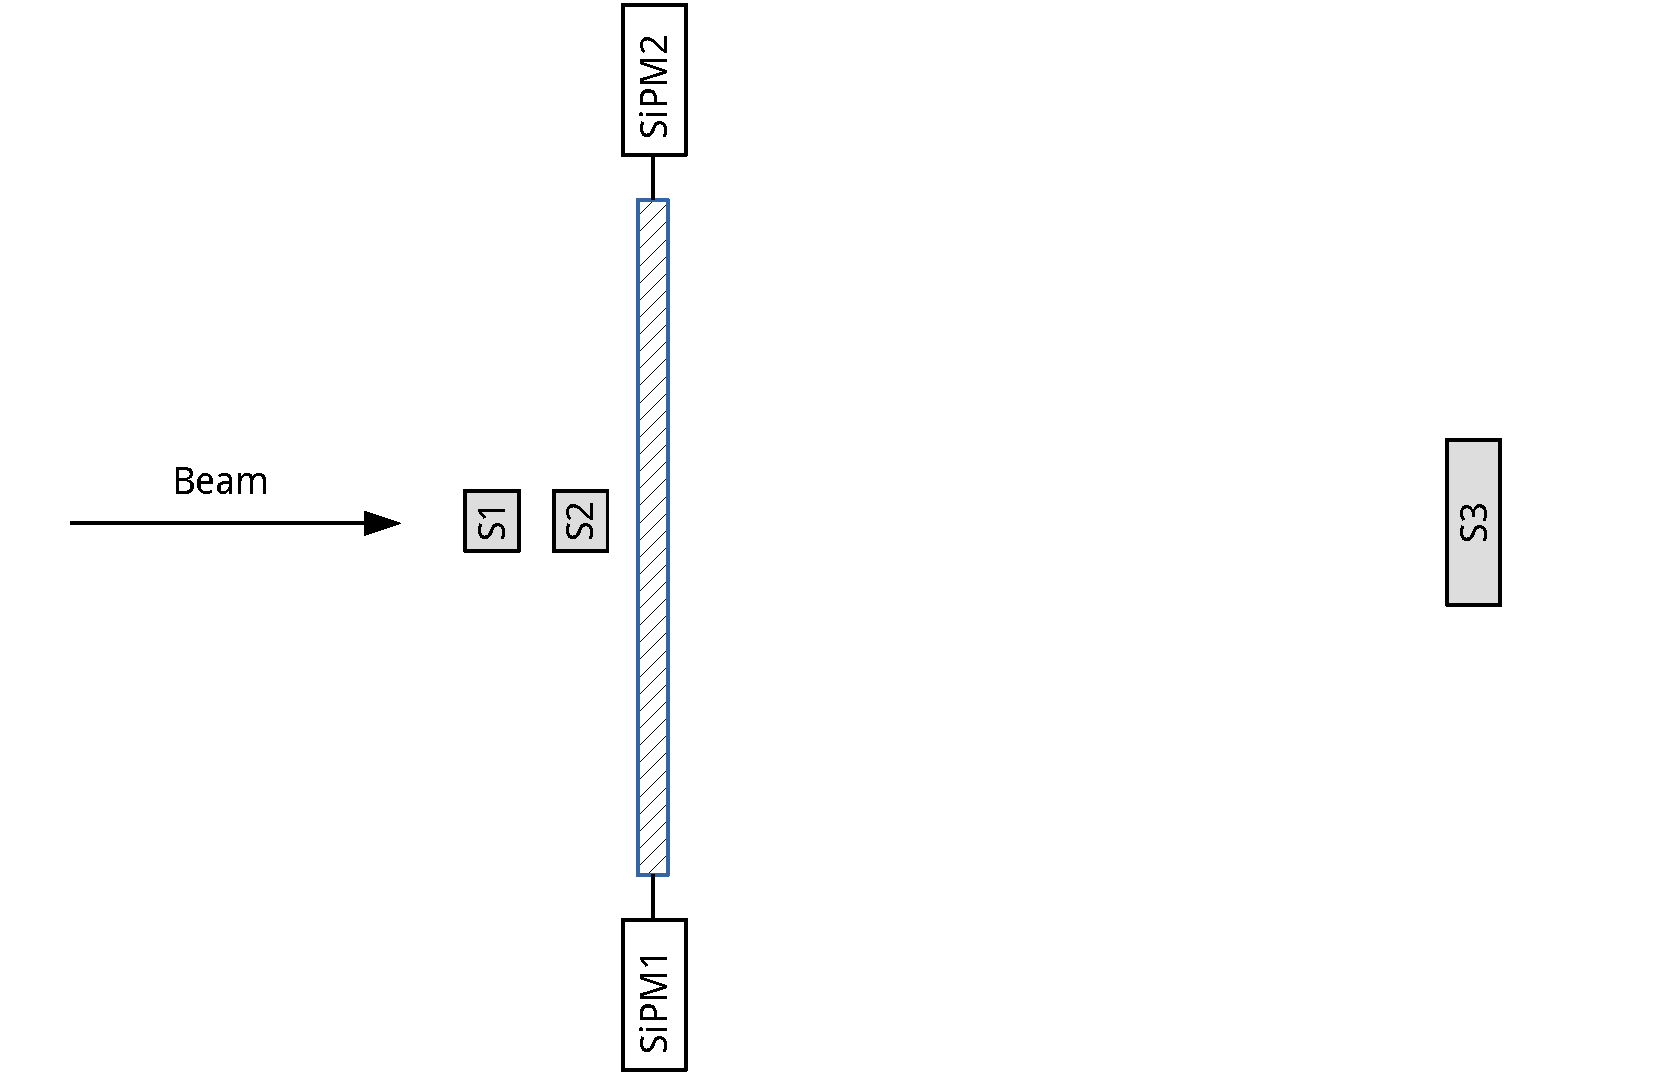
\includegraphics[width=\linewidth,valign=t]{Calorimeter/SiliconTungstenSiD/setup.png}
		\caption{The ECal prototype setup at SLAC, in a silicon-first arrangement.}
		\label{fig:Calorimeter:SiDECAL:setup}
	\end{minipage}
\end{figure}

 In the initial test, a stack of nine silicon sensor planes and eight tungsten plates (corresponding to six radiation lengths) was exposed to beam. Data was taken over a four-day period with a  beam rate between 0.5 and 5 electrons per pulse. The beam was concentrated in a small area of the stack, with mean separation of two electron events of \SIrange{15}{20}{mm}. This data collection provides good measurements of multiple particle overlap and reconstruction of overlapping showers\cite{Steinhebel:2017qze}. Figure~\ref{fig:Calorimeter:SiDECAL:combo} shows the measured total charge distribution for two of the exposure runs compared to a GEANT4 simulation. The distribution was best fit to the simulation assuming a Poisson distribution of beam particles with an average of
0.87. Comparison of the deposited energy distribution in each of the nine layers also agrees well with the simulations.

\begin{figure}
	\centering
	\begin{minipage}[b]{.49\textwidth}
		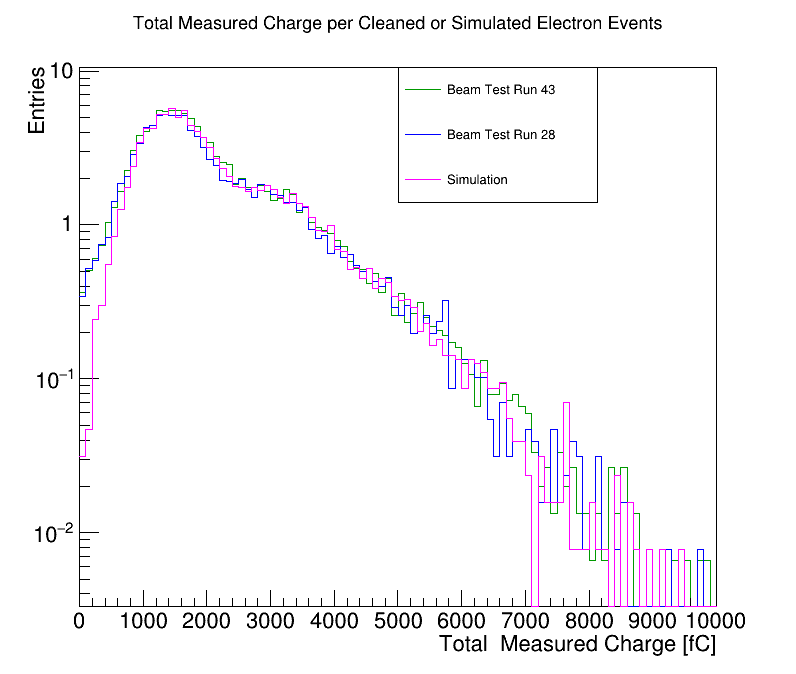
\includegraphics[width=\linewidth,valign=t]{Calorimeter/SiliconTungstenSiD/combo.png}
		\caption{Prototype runs match very well with GEANT4 simulated data.}
		\label{fig:Calorimeter:SiDECAL:combo}
	\end{minipage}\hfill
	\begin{minipage}[b]{.49\textwidth}
		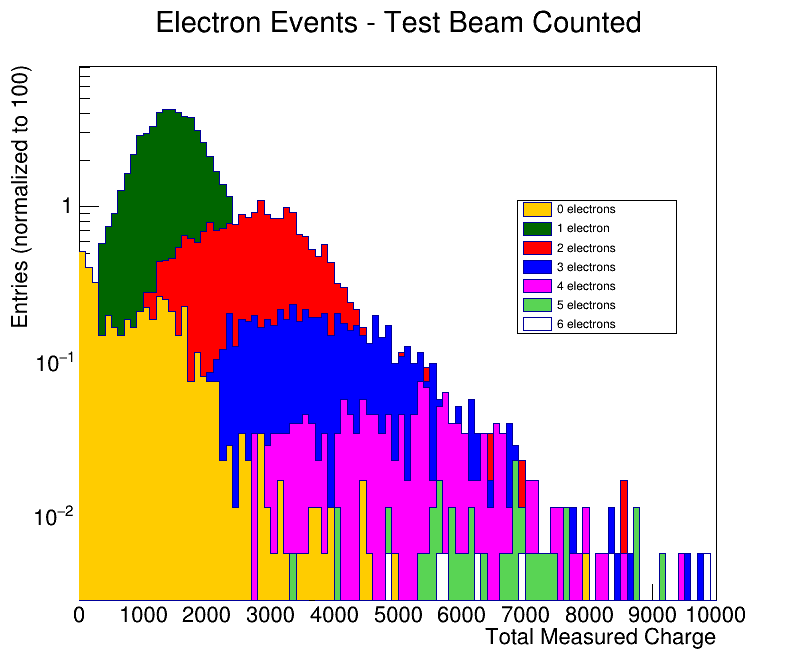
\includegraphics[width=\linewidth,valign=t]{Calorimeter/SiliconTungstenSiD/tbTagged.png}
		\caption{Distributions of the number of counted electrons.}
		\label{fig:Calorimeter:SiDECAL:tbTagged}
	\end{minipage}
\end{figure}

An algorithm was developed to count the number of incident electrons in each event, based on the total and distribution of energy in each of the nine test beam layers. The algorithm counting was verified with simulated events. Figure~\ref{fig:Calorimeter:SiDECAL:tbTagged} shows the test beam distribution of total energy in the nine layers for each of the counted number of events. The analysis was used to assess the ability of the calorimeter to separate two showers as a function of the separation of the showers. Figure~\ref{fig:Calorimeter:SiDECAL:efficiency} presents the two shower separation efficiency versus separation distance, with 100\% efficiency achieved for $>\SI{10}{mm}$ separation.

\begin{figure}
	\centering
	\begin{minipage}[b]{.49\textwidth}
		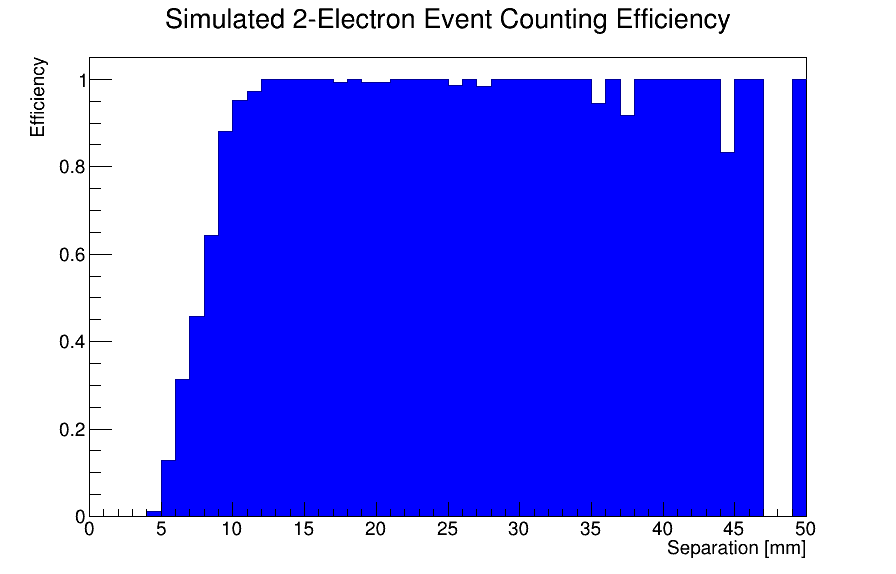
\includegraphics[width=\linewidth,valign=t]{Calorimeter/SiliconTungstenSiD/efficiency.png}
		\caption{Efficiency of electron counting algorithm with simulated two electron events.}
		\label{fig:Calorimeter:SiDECAL:efficiency}
	\end{minipage}\hfill
	\begin{minipage}[b]{.49\textwidth}
		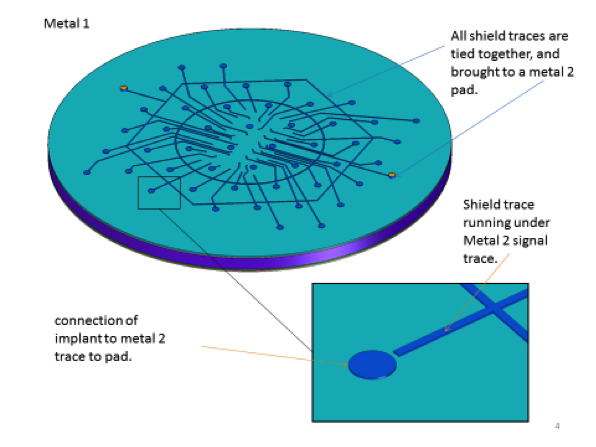
\includegraphics[width=\linewidth,valign=t]{Calorimeter/SiliconTungstenSiD/shield.png}
		\caption{Schematic of the shielded sensor.}
		\label{fig:Calorimeter:SiDECAL:shield}
	\end{minipage}
\end{figure}

\subsection{Engineering Challenges}
The first sensors had aluminum pads which required extensive processing to build the Under Bump Metallization (UBM). The sensor foundry now provides the complete UBM, and the bump bonding process (with the KPiX foundry providing the UBM and eutectic solder balls on KPiX) is relatively straightforward.

 Electromagnetic showers can hit a large number of pixels simultaneously. This causes a disturbance in KPiX as many pixels are reset, resulting in a cascade of increasing multiplicity. This problem is understood and requires a small change in KPiX.

 The sensors have traces that cross over other pixels, which is necessary for a small Read Out Chip on the sensor. We have observed crosstalk due to these parasitic couplings, and have designed a new sensor with shielded traces (Figure~\ref{fig:Calorimeter:SiDECAL:shield}). Both the old and new sensors have a metal 1 connection to the diode by a via to metal 2 traces and to the KPiX. In the old version, the metal 1 contact covered the full area of the diode; in the new version, there is only a small connection to the diode, and metal 1 traces run under the metal 2 traces. The metal 1 traces are tied together and held at fixed potential. These sensors have been fabricated and are now being tested.

 Early versions of the sensor cables were bump bonded to the sensor. While this technique uses the least gap height possible, it was too difficult to use efficiently. New cables have been designed that use wire bonded connections, with separate cables for each sensor.

 The forward calorimeters BEAMCAL and LUMICAL have higher occupancy than the barrel and endcaps. It has long been known that the BEAMCAL has an occupancy of about 1, and will use the BEAN\cite{6200898} chip. Studies with Guinea Pig\cite{LCC-0125} pairs only indicate that the LUMICAL may need a readout with more than 4 buffers of KPiX. KPiX will be studied to see if more buffers can be added.

\subsection{Future Plans}
The SiD silicon-tungsten ECal development has been the result of a collaboration of the SLAC National Accelerator Laboratory and the University of Oregon. R\&D has been constrained by a low level of support, so the ECal progress has been limited and slow. Nevertheless, there is now a pre-conceptual mechanical design. The beam test demonstrated expected behavior from the prototype sensors, but also showed significant crosstalk issues in both the sensor and KPiX. There is now a second sensor prototype with trace shielding that is being tested. The KPiX issues are understood, but a new prototype has not yet been built. Evaluation of expected forward multiplicities is ongoing, and may influence the evolution of KPiX.
Final optimization 
of the ECal (layer configuration and number, etc.) will be finished when funding materializes.

%4.4.5   Acknowledgements
%Work supported by the U.S. Department of Energy under contract number DE-AC02-76SF00515 and award number DE-%SC0017996.
